\section{A GAN for 3D Human Pose Estimation}
\label{sec:network}
In their work "Can 3D Pose Be Learned from 2D Projections Alone?" \citet{drover18} propose a weakly supervised 3D human pose estimation system.
It makes use of a Generative Adversarial Network and can be trained without explicit supervision, meaning that no 3D ground truth poses are required.
The objective of this section is to present and discuss this system in detail, as it provides the foundation of this thesis.
In a first step towards this, Generative Adversarial Networks and perspective projection are  briefly explained.

\subsection{Generative Adversarial Networks}
Generative Adversarial Networks (GANs) have first been presented by \citet{goodfellow14} in 2014.
As the name suggests, they are generative models involving two adversary agents, a \emph{generator} and a \emph{discriminator}.
The generator $G$ is a function that maps elements from a latent distribution $p_z$ to the distribution $p_{fake}$.
The discriminator $D$ tries to determine whether its input belongs to the real data distribution $p_{real}$ (the distribution to be learned) or to the distribution $p_{fake}$.
During training, the generator tries to adjust its internal parameters such that $p_{fake}$ resembles $p_{real}$ as closely as possible, and thus tries to fool the discriminator into thinking that the data produced by it belongs to $p_{real}$.
Meanwhile, the discriminator learns to distinguish between the two distributions.

This procedure can be thought of as two players (the generator and the discriminator) playing a game with value function $V(D, G)$ against each other, where
\begin{equation}
	V(D, G) = \mathbb{E}_{r\sim p_{real}}(\log(D(r))) + \mathbb{E}_{z\sim p_{z}}(\log(1 - D(G(z)))) \ .
\end{equation}
Here, the discriminator tries to maximize the probability of correctly estimating whether the input stems from $p_{real}$ or $p_{fake}$.
The generator simultaneously minimizes the second summand, trying to get the discriminator to classify its output as originating from $p_{real}$.
Thus, GANs can be described as a minimax game with players $G$ and $D$:
\begin{equation}
\min_G \max_D V(D, G) \ .
\end{equation}
\citet{goodfellow14} have shown that this expression takes on its global optimum if and only $p_{fake} = p_{real}$.
In this case, the discriminator produces an output of $\frac{1}{2}$ for all inputs, which means it is no longer able to distinguish between the distributions.

Usually, the generator and the discriminator are two neural networks.
They can be trained with the following loss functions \cite{goodfellow17}:
\begin{align}
\label{eq:generator-loss}
loss_G &= -\mathbb{E}_{z\sim p_{z}}(\log(D(G(z)))) \\
\label{eq:discriminator-loss}
loss_D &= -\frac{1}{2}\mathbb{E}_{r\sim p_{real}}(\log(D(r))) - \frac{1}{2} \mathbb{E}_{z\sim p_{z}}(\log(1 - D(G(z))))
\end{align}
Here, $loss_D$ is the standard cross entropy, as it can be found in a standard (binary) classifier.
The discriminator tries to minimize it during training.
Instead of the generator minimizing the same function with flipped sign, \citet{goodfellow17} suggests flipping the generator's target instead.
This prevents vanishing gradients.
\autoref{eq:generator-loss} describes the resulting loss for the generator.

The advantage of GANs compared to other generative models is that they can learn distributions in a weakly supervised manner, that is, only elements from the distribution to be learned are required for training.
In the system presented by \citet{drover18} that distribution captures all human \emph{2D} poses, which will be further explained in \autoref{sec:network-architecture}.

\subsection{Perspective Projection}

\begin{figure}
	\Todo[inline]{Add figure!}
	\caption{Camera setup used for the theoretical analysis.}
	\label{fig:camera-projection-setup}
\end{figure}

Throughout this thesis, human poses will be projected from three dimensional space into two dimensions and vice versa.
For this projection the simplified model of a pinhole camera is utilized. 
Its only intrinsic parameter, in this case, is a focal length $f$.
The camera has its center of projection at $(0, 0, 0)$, with the virtual image plane being located at $(0, 0, f)$, in parallel to the x-y-plane.
The camera is looking towards positive infinity along the z axis.
The projection from 3D to 2D can be described by the perspective projection equation:
\begin{equation}
	\label{eq:perspective-projection}
	p = 
	\begin{pmatrix}
	x\\
	y
	\end{pmatrix}
	= \frac{f}{Z} \cdot 	
	\begin{pmatrix}
	X\\
	Y
	\end{pmatrix} \ ,
\end{equation}
where $P = (X, Y, Z)$ is a is a three dimensional point in the camera's coordinate system and $p = (x, y)$ the projected point on the (virtual) image plane.
Note that the projection is only defined for points that have $Z \neq 0$.
$Z = 0$ would mean the point is in the same x-y-plane as the center of projection.
However, this issue will be taken care of by ensuring that the there is always enough distance between the 3D points and the camera.
A visualization of a simplified form of the projection is depicted in \autoref{fig:camera-projection-setup}.

Similarly to the projection from three dimensions into two, a 2D point on the image plane $(x, y)$ can also be re-projected into 3D if the depth $Z$ of the point is given.
This re-projection is described by
\begin{equation}
	\label{eq:perspective-re-projection}
	\begin{pmatrix}
	X\\
	Y
	\end{pmatrix} = \frac{Z}{f} \cdot
	\begin{pmatrix}
	x\\
	y
	\end{pmatrix} \ ,
\end{equation}
and the 3D point $P$ in then again given by $(X, Y, Z)$.

\subsection{Network Architecture}
\label{sec:network-architecture}

\begin{figure}
	\centering
	\makebox[\textwidth][c]{
		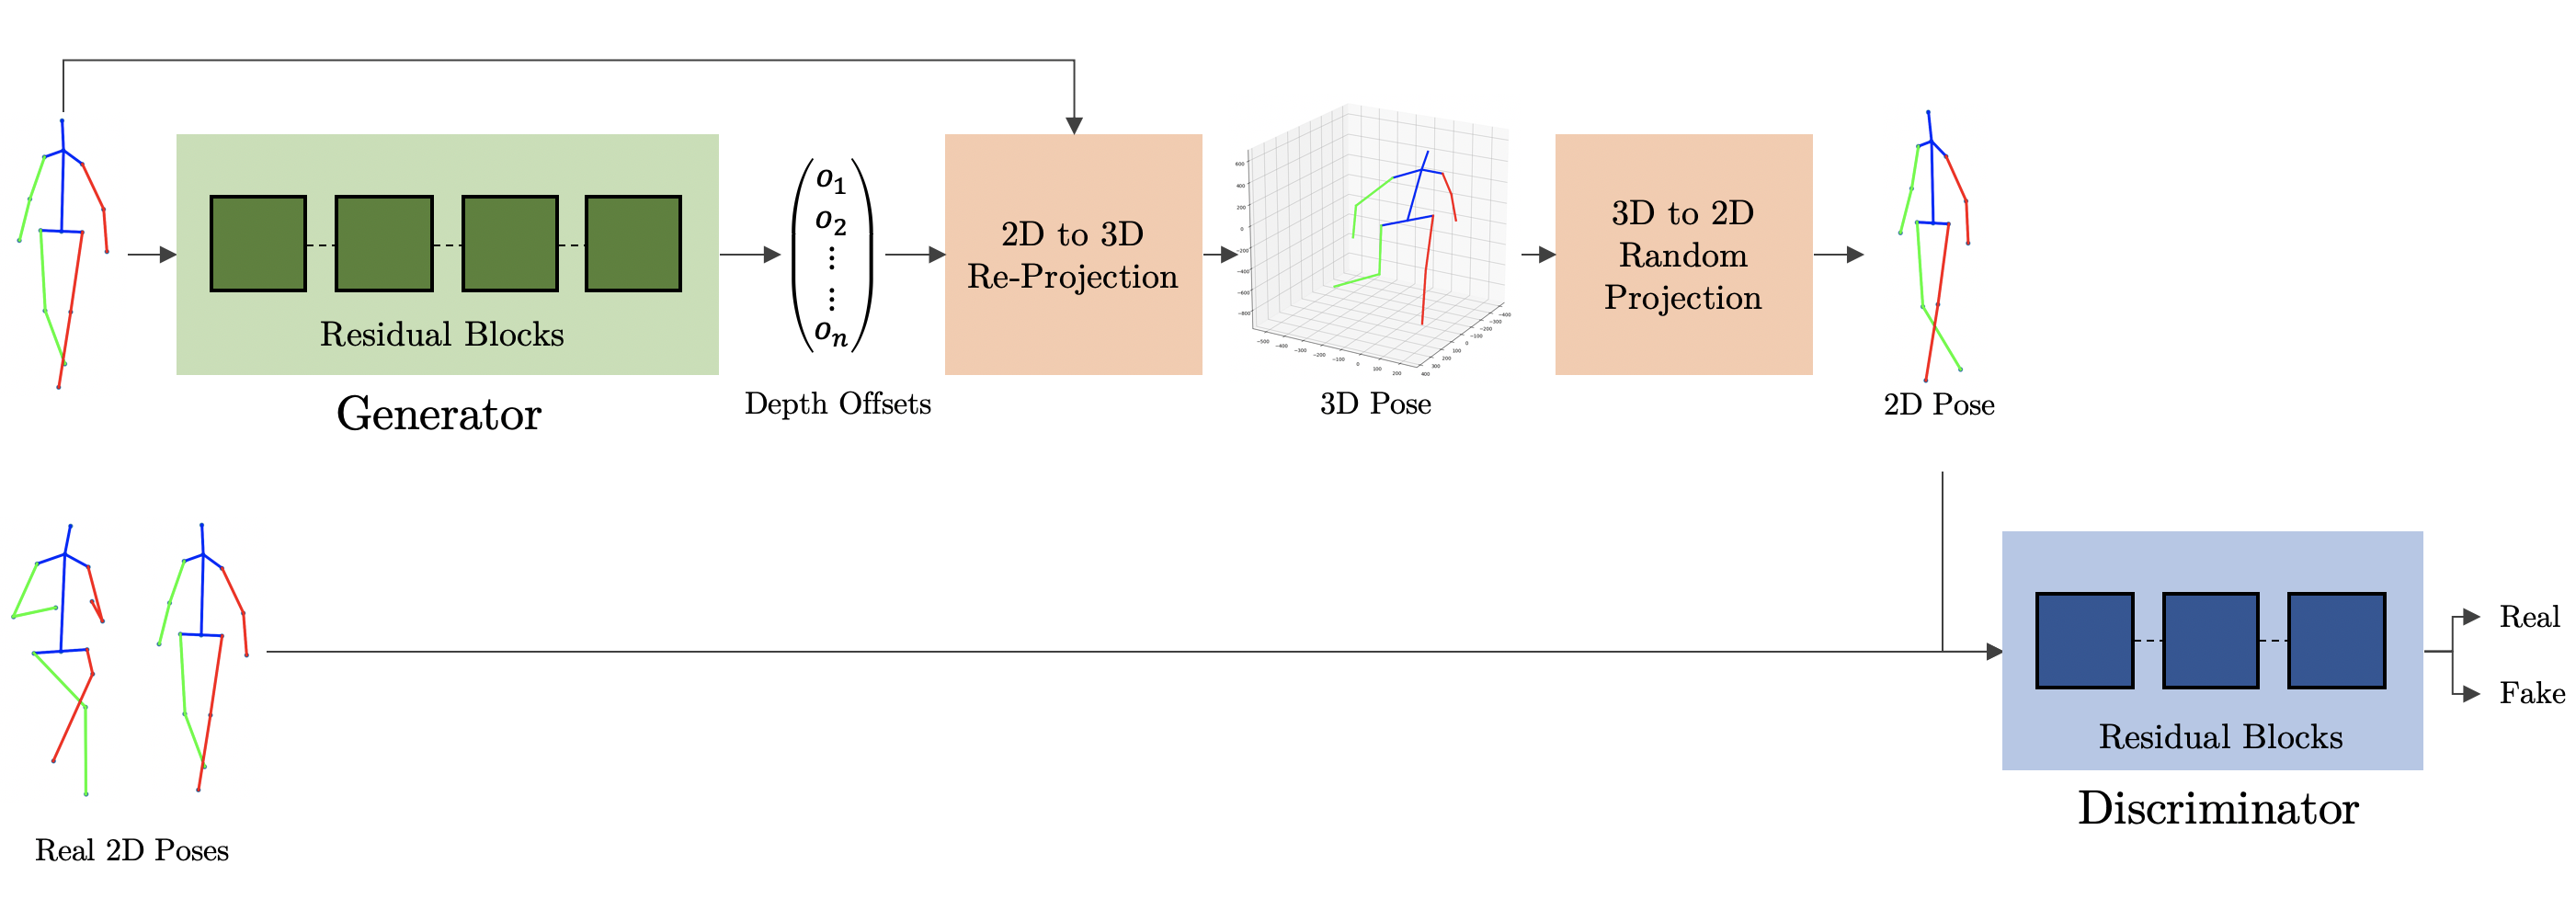
\includegraphics[width=1.1\textwidth]{figures/system.png}
	}
	\caption{The core of this thesis: The 2D to 3D pose GAN proposed by \citet{drover18}.}
	\label{fig:system}
\end{figure}

In their work, \citet{drover18} make use of a GAN in the context of 3D human pose estimation.
\autoref{fig:system} displays a diagram of their proposed system.
It follows the basic GAN architecture and adds some extra layers after the generator.
The architecture will be explained in the following.

In the system, the latent and the real distribution $p_z$ and $p_{real}$ are both the distribution of real 2D poses.
This means that the generator is ultimately also trying to learn that distribution.
On the way to doing that, 3D human poses are created as a byproduct, which can then be used in other applications.

The generator's and discriminator's input are human 2D poses.
During the application of the system, the generator's input pose will the pose to be lifted to 3D.
For numerical stability, \citet{drover18} require the input poses for both discriminator and generator to be normalized in the following way:
\begin{enumerate}[label=(\Alph*)]
	\item The 2D poses' root joint is centered at the origin of the image plane.
	\item A designated norm limb has length $0.1$.
\end{enumerate}
In this work, the root joint is always the pelvis (the center point between the hips) and the norm limb the connection between pelvis and thorax (the spine).

The generator receives 2D poses as input.
For those poses, it estimates the depth of each joint.
In order to eliminate the additional degree of freedom introduced by the scale-distance ambiguity (a 3D pose $P$ and a 3D pose $P'$ twice as far away from the camera and twice as big both project to the same 2D pose), the system aims to estimate 3D poses that have a norm limb length of $1$.
Hence, instead of an absolute depth, only a \emph{depth offset} $o_i$ is estimated for each joint $(x_i, y_i)$.
The absolute depths can then be calculated as
\begin{equation}
	\label{eq:depth-clipping}
	Z_i = \max \{f, Z + o_i\}
\end{equation}
for $1 \leq i \leq n$.
This clipping ensures that, at the time of re-projection to 3D, the points are projected in front of the camera.
In order to obtain a norm limb length of (approximately) $1$, $Z = 10$ has been chosen.
Using the so found depths for each joint, the 2D pose can be re-projected into three dimensions using \autoref{eq:perspective-re-projection}.

Afterwards, the obtained 3D poses are fed to a \emph{Random Projection Layer}, where they are projected to two dimensions again.
For this, the poses are randomly rotated with with azimuth angles between $0$ and $360$ degrees and elevation angles between $0$ and $20$ degrees first and then projected with cameras centered at the root joint with a camera-root-joint-distance of $10$ as in \autoref{eq:perspective-projection}.
The particular choice of elevation angles is based on the heuristic that in reality, people are rather photographed from above than from below.
After the projection, the 2D poses are fed to the discriminator.

During training, the discriminator receives 2D poses from $p_{real}$ and $p_{fake}$ and tries to classify them as either real or fake, that is, as originating from $p_{real}$ or $p_{fake}$.

This system design is based on one underlying heuristic:\vspace{.5em}\newline
\vspace{.5em}
\noindent{\emph{If a random projection of a 2D pose looks realistic, the 3D pose is realistic.}}\newline
This heuristic is based on the fact that it is extremely unlikely for a malformed 3D pose to result in a realistic 2D pose when photographed from a random point of view.

\begin{figure}
	\centering
	\begin{tikzpicture}
	[
	 block/.style ={rectangle, draw=black, thick, text width=20em, align=center, minimum height=2em}
	]
	\node[] (a) [block] {Fully Connected Layer (1024)};
	\node[below= -1.5\pgflinewidth of a] (b) [block] {ReLU};
	\node[below= -1.5\pgflinewidth of b] (c) [block] {Fully Connected Layer (1024)};
	\node[below= -1.5\pgflinewidth of c] (d) [block] {ReLU};
	\node[below= -1.5\pgflinewidth of d] (e) [block] {$\bigoplus$};
	\node[above=of a] (x) [] {};
	\draw[->, line width=1pt] (x) -- (a);
	\node[below=of e] (y) [] {};
	\draw[->, line width=1pt] (e) -- (y);
	\node[above=.4 of a] (z) [] {};
	\node[right=12em of z] (h) [] {};
	\draw[line width=1pt] (z.center) -- (h.center);
	\draw[->, line width=1pt] (h.center) |- (e.east);
	\end{tikzpicture}
	\caption{Architecture of the Residual Blocks in generator and discriminator.
	Two fully connected layers of size 1024 are each followed by a Rectified Linear Unit (ReLU). After the last ReLU the input is added to the output.
	\citet{drover18} suggest a Batch Normalization immediately after each Fully Connected Layer, which has not been found to work.}
	\label{fig:residual-block}
\end{figure}

In practice, both generator and discriminator are neural networks that consist of several consecutive \textit{Residual Blocks}.
A Residual Block consists of two fully connected layers of size $1024$ each followed by Rectified Linear Units (ReLU) and a residual connection adding the input to the last layer's output (\autoref{fig:residual-block}).
In their work, \citet{drover18} describe two additional Batch Normalization layers \cite{ioffe15}, one immediately after each fully connected layer.
Practical tests have shown that when using those additional layers the training does not converge at all.
\unsure{Should I still mention the "personal communication"? I'm not sure if their paper is related to this work enough.}
As competitive results could also be achieved with the reduced network design, the proposed Batch Normalization Layers have been left out completely in this work.

Architecture-wise, the generator takes $n$ 2D joint locations (i.e. $2n$ scalar inputs) as input and feeds them to a fully connected layer of size 1024.
This is followed by four Residual Blocks and concluded by another fully connected layer of size 1024 mapping the output of the last residual block to a vector of size $n$, in which each entry represents the depth offset one joint.

The discriminator's architecture is very similar to the generator's. 
It also accepts $n$ 2D joint locations as input which are fed into a fully connected layer of size 1024, followed by three residual blocks.
The output is then reduced by another fully connected layer to a vector of size 2.
Finally, softmax is applied.
The resulting values imply the probability of the input being either real or fake.

The networks are trained with the standard GAN losses described in Equations~\ref{eq:generator-loss} and~\ref{eq:discriminator-loss}.